\section{Tập hợp}

\subsection{Đề 1}
\Opensolutionfile{ans}[ans/ans-0-B1]
\caulc
\Opensolutionfile{ans}[ans/0-D1-B2]
%=====================================
\begin{ex} %[0D1N2-2]
	Cho tập hợp $X=\{0 ; 2 ; 5\}$. Tập hợp nào dưới đây không phải là tập con của tập hợp $X$?
	\choice
	{$\varnothing$}
	{$\{2\}$}
	{$\{0 ; 2 ; 5\}$}
	{\True  $\{0 ; 1 ; 2\}$}
	\loigiai{
		Ta có $\{1\} \notin X$,  vậy $\{0 ; 1 ; 2\} \not \subset\{0 ; 2 ; 5\}$.
	}
\end{ex}
%=====================================
\begin{ex}%[0D1H3-1]
	Cho tập $A=\{0 ; 2 ; 4 ; 6 ; 8\}$; $B=\{3 ; 4 ; 5 ; 6 ; 7\}$. Tập $A \setminus B$ là
	\choice
	{$\{0 ; 6 ; 8\}$}
	{\True $\{0 ; 2 ; 8\}$}
	{$\{3 ; 6 ; 7\}$}
	{$\{0 ; 2\}$}
	\loigiai{
		Vì $A \setminus B$ gồm các phần tử thuộc tập hợp $A$ và không thuộc $B$ nên $A \setminus B=\{0 ; 2 ; 8\}$.
	}
\end{ex}
%=====================================
\begin{ex}%[0D1H3-1]
	Cách viết nào sau đây là \textbf{sai}?
	\choice
	{$(0 ;+\infty)=\{x \in \mathbb{R}, x>0\}$}
	{$[0 ; 5]=\{x \in \mathbb{R}, 0 \leqslant x \leqslant 5\}$}
	{$(0 ; 5)=\{x \in \mathbb{R}, 0<x<5\}$}
	{\True $[-1 ; 5)=\{-1 ; 0 ; 1 ; 2 ; 3 ; 4\}$}
	\loigiai{
		Vì $[-1 ; 5)=\{x \in \mathbb{R} \mid-1 \leqslant x<5\}$ nên cách viết sau là sai: \lq\lq$[-1 ; 5)=\{-1 ; 0 ; 1 ; 2 ; 3 ; 4\}$\rq\rq.
	}
\end{ex}
%=====================================
\begin{ex}%[0D1N2-1]
	Cho tập hợp $A=\{x+1 \mid x \in \mathbb{N}, x \leq 5\}$. Số phầ tử của tập hợp $A$ là
	\choice
	{$8$}
	{$7$}
	{$5$}
	{\True $6$}
	\loigiai{
		$A=\{x+1 \mid x \in \mathbb{N}, x \leq 5\} \Leftrightarrow A=\{1 ; 2 ; 3 ; 4 ; 5 ; 6\}$. Do đó số phần tử của tập hợp $A$ là $6$.
	}
\end{ex}
%=====================================
\begin{ex}%[0D1H2-1]
	Trong các tập hợp sau,  tập hợp nào là tập hợp rỗng?
	\choice
	{$A=\{x \in \mathbb{Z}|~| x|<1\}$}
	{$B=\left\{x \in \mathbb{Z} \mid 6 x^2-7 x+1=0\right\}$}
	{\True $C=\left\{x \in \mathbb{Q} \mid x^2-4 x+2=0\right\}$}
	{$D=\left\{x \in \mathbb{R} \mid x^2-4 x+3=0\right\}$}
	\loigiai{
		$x^2-4 x+2=0 \Leftrightarrow \hoac{& x=2+\sqrt{2} \notin \mathbb{Q}  \\&  x=2-\sqrt{2} \notin \mathbb{Q}} \Rightarrow C=\varnothing$.
	}
\end{ex}
%=====================================
\begin{ex}%[0D1N1-2]
	Cho $x$ là một phần tử của tập hợp $X$. Mệnh đề nào sau đây là đúng?
	\choice
	{\True $x \in X$}
	{$X \in x$}
	{$x \subset X$}
	{$\{x\} \in X$}
	\loigiai{
		Mệnh đề là đúng là $x \in X$. Kí hiệu $x$ là một phần tử của tập hợp $X$.
	}
\end{ex}
%=====================================
\begin{ex}%[0D1H2-2]
	Số tập con của tập $C=\{x \in \mathbb{Z} \mid-1 \leqslant x \leqslant 1\}$ là
	\choice
	{$3$}
	{$2$}
	{\True $8$}
	{$6$}
	\loigiai{
		Ta có $C=\{-1 ; 0 ; 1\}$.\\
		Số tập con của tập $C$ là $2^3=8$.
	}
\end{ex}
%=====================================
\begin{ex}%[0D1H3-4]
	Cho tập hợp $A=\{x \in \mathbb{R} \mid 2 \leqslant x<5\}$. Phần bù của tập hợp $A$ trong $\mathbb{R}$ là tập nào sau đây?
	\choice
	{$[5 ;+\infty)$}
	{$(-\infty ; 2)$}
	{$(-\infty ; 2] \cup(5 ;+\infty)$}
	{\True $(-\infty ; 2) \cup[5 ;+\infty)$}
	\loigiai{
		Phần bù của tập hợp $A$ trong $\mathbb{R}$ là $\mathrm{C_{\mathbb{R}}A}=(-\infty ; 2) \cup[5 ;+\infty)$.
	}
\end{ex}
%=====================================
\begin{ex}%[0D1V3-3]
	Cho tập hợp $A=(0 ;+\infty)$ và $B=\left\{x \in \mathbb{R} \mid m x^2-6 x+m-8=0\right\}$, $m$ là tham số. Biết rằng tập $B$ có đúng hai tập con và $B \subset A$. Kết luận nào sau đây là đúng về giá trị của tham số $m$.
	\choice
	{$m \in(0 ; 9)$ }
	{\True  $m \in(0 ; 10)$}
	{$m \in(0 ; 8)$}
	{$m \in(0 ; 7)$}	
	\loigiai{
		Vì tập $B$ có đúng hai tập con nên phương trình $m x^2-6 x+m-8=0$ có duy nhất một nghiệm.
		\begin{enumerate}[TH1.]
			\item $m=0$ thì $x=-\dfrac{4}{3} \Rightarrow B=\left\{-\dfrac{4}{3}\right\}$.
			\item $m \neq 0$ thì phương trình có nghiệm duy nhất $\Leftrightarrow \Delta'=0$
			$\Leftrightarrow 9-m(m-8)=0$
			$\Leftrightarrow-m^2+8 m+9=0$
			$\Leftrightarrow \hoac{& m=-1  \\&  m=9}$. 
			\begin{itemize}
				\item Với $m=-1 \Rightarrow B=\{-3\}$
				\item Với $m=9 \Rightarrow B=\left\{\dfrac{1}{3}\right\}$
			\end{itemize}
			Kết hợp với điều kiện $B \subset A$ ta có $m=9$.
		\end{enumerate}
	}
\end{ex}
%=====================================
\begin{ex}%[0D1N3-3]
	Cho tập $M=\{x \in R \mid(x+3)(x-1) \geqslant 0\}$ và $N=(m-1 ; m+1]$. Tìm $m$ để $M \cap N \neq \varnothing$
	\choice
	{$ \hoac{& m \leqslant-2  \\&  m>0}$}
	{\True  $ \hoac{& m<-2  \\&  m \geqslant 0}$}
	{$ \hoac{& m \leqslant-2  \\&  m \geqslant 0}$}
	{$-2 \leqslant m<0$}	
	\loigiai{
		Ta có $(x+3)(x-1) \geqslant 0 \Leftrightarrow \hoac{& x \leqslant-3  \\&  x \geqslant 1} $
		$\Rightarrow M=(-\infty ;-3] \cup[1 ;+\infty)$.\\
		Để $M \cap N=\varnothing \Leftrightarrow \heva{& m-1>-3  \\&  m+1<1} \Leftrightarrow \heva{& m>-2  \\&  m<0}\Leftrightarrow-2<m<0$.\\
		Suy ra $M \cap N \neq \varnothing \Leftrightarrow \hoac{& m<-2  \\&  m \geqslant 0}$.
	}
\end{ex}
%=====================================
\begin{ex}%[0D1H3-2]
	\immini{ Cho các tập hợp $A$, $B$, $X$ được biểu diễn trong biểu đồ Ven như sau. Khẳng định nào sau đây \textbf{sai}?
		\choice
		{$B \subset C_X A$}
		{$A \cap B=\varnothing$}
		{$A \subset C_X B$}
		{\True $A \cup B=X$}
	}{
		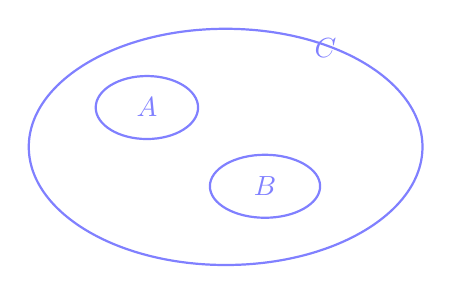
\begin{tikzpicture}[scale=0.5,thick,rotate=-90]
			\colorlet{MauNet}{blue!50}
			\def\ElipA{(0,0) ellipse (0.8cm and 1.3cm)}
			\def\ElipB{(2,3) ellipse (0.8cm and 1.4cm)}
			\def\ElipC{(1,2) ellipse (3cm and 5cm)}
			\draw[MauNet] \ElipA node[blue!50] {$A$};
			\draw[MauNet] \ElipB node[blue!50] {$B$};
			\draw[MauNet] \ElipC node[blue!50,above right=1cm] {$C$};
		\end{tikzpicture}
	}
	\loigiai{
		Nhìn biểu đồ,  ta thấy $A \cup B \neq X$
	}
\end{ex}
%=====================================
\begin{ex}%[0D1H2-3]
	Cho $A=[-1 ; 3]$; $B=(2 ; 5)$. Tìm mệnh đề \textbf{sai}.
	\choice
	{$B \setminus A=(3 ; 5)$}
	{$A \cap B=(2 ; 3]$}
	{$A \setminus B=[-1 ; 2]$}
	{\True  $A \cup B=[-1 ; 5]$}
	\loigiai{
		Ta có $A \cup B=[-1 ; 5)$
	}
\end{ex}
\Closesolutionfile{ans}
\indapan{6}{ans/ans-0-B1}
\cauds
\Opensolutionfile{ans}[ans/ans-0-B1-DS]
\begin{ex}%Câu 1
	Cho các tập hợp 
	\begin{eqnarray*}
		A&=&\{-3 ;-2 ;-1 ; 0 ; 1 ; 2 ; 3\};\\
		B&=&\{0 ; 1 ; 4 ; 5\};\\
		C&=&\{-4 ;-3 ; 1 ; 2 ; 5 ; 6\}
	\end{eqnarray*} Các mệnh đề sau đúng hay sai?
	\choiceTF
	{\True $A\cup B=\{-3 ;-2 ;-1 ; 0 ; 1 ; 2 ; 3 ; 4 ; 5\}$}
	{$A\cap B=\{0\}$}
	{\True $(A\cup B)\cap C=\{-3 ; 1 ; 2 ; 5\}$}
	{\True $A\cap B\cap C=\{1\}$}
	\loigiai{
		\begin{itemchoice}
			\itemch Đúng. Vì $A\cup B=\{-3 ;-2 ;-1 ; 0 ; 1 ; 2 ; 3 ; 4 ; 5\}$.
			\itemch Sai. Vì $A\cap B=\{0 ; 1\}$
			\itemch Đúng. Vì $(A\cup B)\cap C=\{-3 ; 1 ; 2 ; 5\}$.
			\itemch Đúng. Vì $A\cap B\cap C=\{1\}$.
		\end{itemchoice}
	}
\end{ex}

\begin{ex}%Câu 2
	Cho các tập hợp sau 
	\begin{eqnarray*}
		A&=&\left\{ x\in\mathbb{Q}\mid x^2-x-6=0\right\};\\
		B&=&\left\{ x\in\mathbb{Z}\mid x^4-11x^2+18=0\right\};\\
		C&=&\left\{x\in\mathbb{N}\mid \left(x^2-3x-10\right)\left(5x^3-6x^2+x\right)=0\right\};\\
		D=\left\{ x\in\mathbb{Z}\mid-2<3x+7\le 10\right\}.
	\end{eqnarray*} Khi đó
	\choiceTF
	{Tập hợp $A$ có $2$ phần tử}
	{Tập hợp $B$ có $3$ phần tử}
	{Tập hợp $C$ có $2$ phần tử}
	{Tập hợp $D$ có $4$ phần tử}
	\loigiai{
		\begin{itemchoice}
			\itemch $x^2-x-6=0\Leftrightarrow\hoac{&x=-2\in\mathbb{Q}\\& x=3\in\mathbb{Q}.}$\\ Vậy $A=\{-2 ; 3\}$.
			\itemch $x^4-11 x^2+18=0\Leftrightarrow\hoac{&x^2=2\\& x^2=9}\Leftrightarrow\hoac{&x=\sqrt{2}\notin\mathbb{Z}\\& x=-\sqrt{2}\notin\mathbb{Z}\\& x=3\in\mathbb{Z}\\& x=-3\in\mathbb{Z}.}$\\Vậy $B=\{-3 ; 3\}$.
			\itemch $\left(x^2-3 x-10\right)\left(5 x^3-6 x^2+x\right)=0\Leftrightarrow \hoac{&x^2-3 x-10=0\\& 5 x^3-6 x^2+x=0}\Leftrightarrow\hoac{&x=5\in\mathbb{N}\\& x=-2\notin\mathbb{N}\\& x=0\in\mathbb{N}\\& x=1\in\mathbb{N}\\& x=\dfrac{1}{5}\notin\mathbb{N}.}$\\
			Vậy $C=\{0 ; 1 ; 5\}$.
			\itemch $-2<3 x+7\leq 10\Leftrightarrow-3<x\leq 1$. Mà $x\in\mathbb{Z}\Rightarrow x\in D=\{-2; -1; 0; 1\}$. Vậy $D$ có $4$ phần tử.
	\end{itemchoice}}
\end{ex}

\begin{ex}%Câu 3
	Lớp $10 B_1$ có 7 học sinh giỏi Toán, 5 học sinh giỏi Lý, 6 học sinh giỏi Hóa, 2 học sinh chỉ giỏi Toán và Lý, 3 học sinh chỉ giỏi Toán và Hóa, 1 học sinh chỉ giỏi cả Lý và Hóa, 1 học sinh giỏi cả 3 môn Toán, Lý, Hóa. Các mệnh đề sau đúng hay sai?
	\choiceTF
	{ Số học sinh chỉ giỏi môn Toán là $1$ học sinh}
	{Số học sinh chỉ giỏi môn Lý là $1$ học sinh}
	{Số học sinh chỉ giỏi môn Hóa là $2$ học sinh}
	{Số học sinh giỏi ít nhất một môn (Toán, Lý, Hóa) là $10$ học sinh}
	\loigiai{
		\begin{itemchoice}
			\itemch Số học sinh chỉ giỏi môn Toán $7-3-1-2=1$.
			\itemch Số học sinh chỉ giỏi môn Lý $5-1-1-2=1$.
			\itemch Số học sinh chỉ giỏi môn Hóa $6-3-1-1=1$.
			\itemch Số học sinh giỏi ít nhất một môn (Toán, Lý, Hóa) là: $1+2+1+1+1+3+1=10$.
	\end{itemchoice}}
\end{ex}

\begin{ex}%Câu 4
	Cho ba tập hợp $A=\{2; 5\}$, $B=\{5 ; x\}$, $C=\{x ; y ; 5\}$, biết $A=B=C$. Khi đó
	\choiceTF
	{$x=y=2$ thì $A=B=C$}  
	{$x=y=3$ thì $A=B=C$}
	{$x=2$, $y=5$ thì $A=B=C$}
	{$x=1$, $y=3$ thì $A=B=C$}
	\loigiai{
		\begin{itemchoice}
			\itemch Đúng. Vì $A=B$ nên $x=2$. Lại có $B=C$ nên $y=x=2$ hoặc $y=5$.
			\itemch Sai. Vì $A=B$ nên $x=2$. Lại có $B=C$ nên $y=x=2$ hoặc $y=5$.
			\itemch Vì $A=B$ nên $x=2$. Lại có $B=C$ nên $y=x=2$ hoặc $y=5$.
			\itemch Sai. Vì $A=B$ nên $x=2$. Lại có $B=C$ nên $y=x=2$ hoặc $y=5$.
		\end{itemchoice}	
		Vậy $x=y=2$ hoặc $x=2, y=5$.}
\end{ex}

\Closesolutionfile{ans}
\indapan{3}{ans/ans-0-B1-DS}

\Opensolutionfile{ans}[ans/ans-0-B1-KQ]
\caukq
\begin{bt}%[0D1H3-5]
	Lớp 10A có $45$ học sinh trong đó có $12$ bạn học sinh giỏi Văn, $ 9$ bạn học sinh giỏi Địa lí, và $30$ bạn không giỏi môn học nào trong hai môn Văn, Địa lí. Hỏi lớp 10A có bao nhiêu bạn học sinh giỏi cả hai môn Văn và Địa lí?
	\shortans{$6$}
	\loigiai{
		\immini{Số học sinh giỏi văn hoặc giỏi địa lí là $45 - 30=15$ (học sinh).\\
			Số học sinh giỏi cả 2 môn văn và địa lí là: $12+9-15=6$ (học sinh)}	
		{\begin{tikzpicture}
				\draw (-3,-1.5) rectangle (3,3);
				\draw (-1,1) circle(1.41) (1,1)circle (1);
				\draw (0,-1)node[below]{$\tiny{\text{30 học sinh không giỏi Văn và Địa} }$} ;
				\draw (-1,1.5)node[below]{$\tiny{\text{12 HS giỏi Văn}}$ } ;
				\draw (1.15,1)node[below]{$\tiny{\text{9 HS giỏi Địa}}$ } ;
				\draw (0,3.5)node[below]{$\tiny{\text{Lớp 10A có 45 học sinh}}$ } ;
		\end{tikzpicture}}		
	}
\end{bt}
%=====================================
\begin{ex}%[0D1V3-3]	
	Cho tập hợp $A=(-\infty ; 1)$, $B=\left[m^2-3 ;+\infty\right)$. Có bao nhiêu giá trị nguyên của tham số để $A \cap B \neq \varnothing$.
	\shortans{$3$}
	\loigiai{
		$A \cap B \neq \varnothing \Leftrightarrow 1>m^2-3 \Leftrightarrow m^2-4<0 \Leftrightarrow-2<m<2$.
	}
\end{ex}

\begin{ex}%[0D1V2-2]
	Cho tập hợp $A=[4 ; 7]$ và $B=(2 a-1 ; 3 a+5]$ khác tập rỗng, với $a \in R$. Gọi $S$ là tập hợp các giá trị nguyên của $a$ để $A \subset B$. Có bao nhiêu tập con của $S$?
	\shortans{$4$}
	\loigiai{
		\begin{itemize}
			%\item  Vẽ trục số thể hiện $A \subset B$
			\item  Điều kiện tập B khác tập rỗng: $2 a-1<3 a+5 \Leftrightarrow a>-6$\, \hfill{(1)}.
			\item  $A \subset B \Rightarrow \heva{& 2 a-1<4  \\&  3 a+5 \geqslant 7 } \Leftrightarrow \heva{& a<\dfrac{5}{2}  \\&  a \geqslant \dfrac{2}{3}} \Leftrightarrow \dfrac{2}{3} \leqslant a<\dfrac{5}{2}.$ \, \hfill{(2)}.
			\item  Kết hợp $(1)$ và $(2)$, ta được $\dfrac{2}{3} \leqslant a<\dfrac{5}{2}$.
			\item  Xét các giá trị $a \in Z \Rightarrow S=\{1 ; 2\}$
			\item Có $4$ tập con của $S$ là $\varnothing $; $\{1\} $; $\{2\}$ và $S=\{1 ; 2\}$.
		\end{itemize}
	}
\end{ex}
\begin{ex}%[0D1V2-2]
	Cho 2 tập khác rỗng $A=(m-1 ; 4] ; B=(-2 ; 2 m+2)$, $m \in \mathbb{R}$. Tìm $m$ nguyên dương để $A \subset B$.
	\shortans{$3$}
	\loigiai{
		Với $2$ tập khác rỗng $A$, $B$ ta có điều kiện $ \heva{& m-1<4  \\&  2 m+2>-2} \Leftrightarrow \heva{& m<5  \\&  m>-2} \Leftrightarrow-2<m<5$.\\
		Để $A \subset B \Leftrightarrow \heva{& m-1 \geqslant-2  \\&  2 m+2>4} \Leftrightarrow \heva{& m \geqslant-1  \\&  2 m+2>4} \Leftrightarrow \heva{& m \geqslant-1  \\&  m>1} \Leftrightarrow m>1$.
		\\
		So với điều kiện $\Rightarrow 1<m<5$. Do đó có $3$ giá trị của $m$ thì $A\subset B$.
	}
\end{ex}
\begin{ex}%[0D1H3-4]
	Cho hai tập hợp $A=\{n \in \mathbb{N} \mid-2<n \leqslant 4\}$ và $B=\left\{x \in \mathbb{Z} \mid 2 x^3+x^2-x=0\right\}$. Hãy viết Số phần tử của  tập hợp $A \cap B$, $A \setminus B$.
	\shortans{$1$, $4$}
	\loigiai{
		Ta có $A=\{0 ; 1 ; 2 ; 3 ; 4\}$, $B=\{-1 ; 0\}$.\\
		Suy ra $A \cap B=\{0\}$ và $A \setminus B=\{1 ; 2 ; 3 ; 4\}$
	}
\end{ex}
\begin{ex}%[0D1V2-2]
	Cho hai tập hợp khác rỗng $A=(1 ; 5)$ và $B=(m ; 4 m-1)$, $m \in \mathbb{R}$. Có bao nhiêu giá trị nguyên của tham số $m$ để $B \subset A$.
	\shortans{$1$}
	\loigiai{
		Để $B \neq \varnothing $ thì $m<4 m-1 \Leftrightarrow m>\dfrac{1}{3}$ \, \hfill{(1)}.\\
		$ B \subset A \Rightarrow \heva{&m \geqslant 1\\&
			4 m-1\leq 5} \Leftrightarrow 1 \leqslant m \leqslant \dfrac{3}{2}$\, \hfill{(2)}.\\
		Từ $(1)$, $(2)$ suy ra $1 \leqslant m \leqslant \dfrac{3}{2}$ (hay $m \in\left[1 ; \dfrac{3}{2}\right]$).
		Vậy có $1$ giá trị nguyên của $m$ thì $B \subset A$.
	}
\end{ex}
\begin{ex}%[0D1V2-2]
	
	Cho tập hợp $A=[4 ; 7]$ và $B=(2 a-1 ; 3 a+5]$ khác tập rỗng, với $a \in R$. Gọi $S$ là tập hợp các giá trị nguyên của $a$ để $A \subset B$. Số tập con của $S$.
	\shortans{$4$}
	\loigiai{
		\begin{itemize}
			%\item  Vẽ trục số thể hiện $A \subset B$
			\item  Điều kiện tập B khác tập rỗng: $2 a-1<3 a+5 \Leftrightarrow a>-6$\, \hfill{(1)}.
			\item  $A \subset B \Rightarrow \heva{& 2 a-1<4  \\&  3 a+5 \geqslant 7 } \Leftrightarrow \heva{& a<\dfrac{5}{2}  \\&  a \geqslant \dfrac{2}{3}} \Leftrightarrow \dfrac{2}{3} \leqslant a<\dfrac{5}{2}.$ \, \hfill{(2)}.
			\item  Kết hợp $(1)$ và $(2)$, ta được $\dfrac{2}{3} \leqslant a<\dfrac{5}{2}$.
			\item  Xét các giá trị $a \in Z \Rightarrow S=\{1 ; 2\}$
			\item Có $4$ tập con của $S$ là $\varnothing $; $\{1\} $; $\{2\}$ và $S=\{1 ; 2\}$.
		\end{itemize}
	}
\end{ex}
\Closesolutionfile{ans}
\indapan{6}{ans/ans-0-B1-KQ}
\newpage
\subsection{Đề 2}
\Opensolutionfile{ans}[ans/ans-0-B1]
\caulc
\begin{ex}%[0D1N2-3]
	Cho tập hợp $A=\left\{ x\in N|\left( {x^3}-9x \right)\left( 2x^2-5x+2 \right)=0 \right\}.$ Tập $A$ được viết theo kiểu liệt kê là
	\choice
	{$\left\{ 2;3 \right\}$}
	{$\left\{ -3;0;\dfrac{1}{2};2;3 \right\}$}
	{$\left\{ -3;0;2;3 \right\}$}
	{\True $\left\{ 0;2;3 \right\}$}
	\loigiai{		
		$\left( {x^3}-9x \right)\left( 2x^2-5x+2 \right)=0\Leftrightarrow \left[ \begin{aligned}
			& {x^3}-9x=0 \\
			& 2x^2-5x+2=0 \\
		\end{aligned} \right.\Leftrightarrow \left[ \begin{aligned}
			& x=0 \\
			& x=3 \\
			& x=2 \\
		\end{aligned} \right.$}
\end{ex}
\begin{ex}%[0D1N2-3]	
	Cho tập $X=\left\{ x\in \mathbb{N}/\left( {x^2}-4 \right)\left( x-1 \right)\left( {x^2}-7x+3 \right)=0 \right\}$. Tính tổng $S$các phần tử của $X$.
	\choice
	{$S=\dfrac{9}{2}$}
	{$S=5$}
	{\True $S=6$}
	{$S=4$}
	\loigiai{		
		Ta có: $\left\{ \begin{aligned}
			& {x^2}-4=0\Leftrightarrow x=\pm 2 \\
			& x-1=0\Leftrightarrow x=1 \\
			& {x^2}-7x+3=0\Leftrightarrow x=3,x=\dfrac{1}{2} \\
		\end{aligned} \right.$\\
		Do $x\in \mathbb{N}\Rightarrow x\in \left\{ 2;1;3 \right\}\Rightarrow S=6$.}
\end{ex}
\begin{ex}%[0D1N2-3]	
	Liệt kê các phần tử của tập hợp $A=\left\{ x\in \mathbb{N}|\left( 6x^2-7x+1 \right)\left( {x^2}-4 \right)=0 \right\}$ ta được
	\choice
	{$A=\left\{ \dfrac{1}{6};\dfrac{1}{2};2 \right\}.$}
	{$A=\left\{ -2;1;2 \right\}.$}
	{$A=\left\{ -2;\dfrac{1}{6};1;2 \right\}.$}
	{\True $A=\left\{ 1;2 \right\}$}
	\loigiai{		
		Xét phương trình $\left( 6x^2-7x+1 \right)\left( {x^2}-4 \right)=0\Leftrightarrow \left[ \begin{aligned}
			& x=1\in \mathbb{N} \\
			& x=\dfrac{1}{6}\notin \mathbb{N} \\
			& x=2\in \mathbb{N} \\
			& x=-2\notin \mathbb{N} \\
		\end{aligned} \right.$.\\
		Vậy $A=\left\{ 1;2 \right\}.$}
\end{ex}
\begin{ex}%[0D1N2-3]	
	Hãy liệt kê các phần tử của tập $X=\left\{ x\in \mathbb{Q}|\left( {x^2}-x-6 \right)\left( {x^2}-5 \right)=0 \right\}$.
	\choice
	{$X=\left\{ -\sqrt{5};\sqrt{5} \right\}$}
	{$X=\left\{ -\sqrt{5};-2;\sqrt{5};3 \right\}$}
	{\True $X=\left\{ -2;3 \right\}$}
	{$X=\left\{ \sqrt{5};3 \right\}$}
	\loigiai{		
		Ta có $\left( {x^2}-x-6 \right)\left( {x^2}-5 \right)=0\Leftrightarrow \left[ \begin{aligned}
			& {x^2}-x-6=0 \\
			& {x^2}-5=0 \\
		\end{aligned} \right.\Leftrightarrow \left[ \begin{aligned}
			& x=-2 \\
			& x=3 \\
			& x=\sqrt{5}\notin \mathbb{Q} \\
			& x=-\sqrt{5}\notin \mathbb{Q} \\
		\end{aligned} \right.$.\\
		Do vậy $X=\left\{ -2;3 \right\}$.}
\end{ex}
\begin{ex}%[0D1N2-3]	
	Kí hiệu nào sau đây dùng để viết đúng mệnh đề $''\sqrt{2}$ không phải là số hữu tỉ$''$?
	\choice
	{$\sqrt{2}\subset \mathbb{Q}$}
	{\True $\sqrt{2}\notin \mathbb{Q}$}
	{$\sqrt{2}\ne \mathbb{Q}$}
	{$\sqrt{2}\in \mathbb{Q}$}
	\loigiai{
		$\sqrt{2}\notin \mathbb{Q}$}
\end{ex}
\begin{ex}%[0D1N2-3]	
	Trong các tập hợp sau, tập nào là tập rỗng?
	\choice
	{$\left\{ \left. x\in \mathbb{R} \right|x^2+5x-6=0 \right\}$}
	{$\left\{ \left. x\in \mathbb{Q} \right|3x^2-5x+2=0 \right\}$}
	{\True $\left\{ \left. x\in \mathbb{Z} \right|x^2+x-1=0 \right\}$}
	{$\left\{ \left. x\in \mathbb{R} \right|x^2+5x-1=0 \right\}$}
	\loigiai{		
		Ta có:\\
		$x^2+5x-6=0\Leftrightarrow \left[ \begin{aligned}
			& x=1 \\
			& x=-6 \\
		\end{aligned} \right.$. Vậy $A=\left\{ -6;1 \right\}$.\\
		$3x^2-5x+2=0\Leftrightarrow \left[ \begin{aligned}
			& x=1 \\
			& x=\dfrac{2}{3} \\
		\end{aligned} \right.$. Vậy $B=\left\{ 1;\dfrac{2}{3} \right\}$.\\
		$x^2+x-1=0\Leftrightarrow \left[ \begin{aligned}
			& x=\dfrac{-1+\sqrt{5}}{2} \\
			& x=\dfrac{-1-\sqrt{5}}{2} \\
		\end{aligned} \right.$. Vì $x\in \mathbb{Z}$ nên $C=\varnothing $.\\
		$x^2+5x-1=0\Leftrightarrow \left[ \begin{aligned}
			& x=\dfrac{-5+\sqrt{29}}{2} \\
			& x=\dfrac{-5-\sqrt{29}}{2} \\
		\end{aligned} \right.$. Vậy $D=\left\{ \dfrac{-5+\sqrt{29}}{2};\dfrac{-5-\sqrt{29}}{2} \right\}$.}
\end{ex}
\begin{ex}%[0D1N2-3]	
	Viết tập hợp $A=\left\{ x\in \mathbb{N}\left| \left( 2x+1 \right) \right.\left( {x^2}-5x+6 \right)=0 \right\}$ bằng cách liệt kê.
	\choice
	{$\left\{ -1;2;3 \right\}$}
	{\True $\left\{ 2;3 \right\}$}
	{$\left\{ -\dfrac{1}{2};2;3 \right\}$}
	{$\left\{ -1;2 \right\}$}
	\loigiai{
		
		Ta có $\left( 2x+1 \right)\left( {x^2}-5x+6 \right)=0\Leftrightarrow \left[ \begin{aligned}
			& 2x+1=0 \\
			& {x^2}-5x+6+0 \\
		\end{aligned} \right.\Leftrightarrow \left[ \begin{aligned}
			& x=-\dfrac{1}{2} \\
			& x=2 \\
			& x=3 \\
		\end{aligned} \right.$.\\
		Do $x\in \mathbb{N}\Rightarrow A=\left\{ 2;3 \right\}$.}
\end{ex}
\begin{ex}%[0D1N2-3]	
	Cho mệnh đề $A=\left\{ x\in Q|\left( x+1 \right)\left( x-\dfrac{1}{2} \right)\left( {x^2}-2 \right)=0 \right\}$. Viết lại tập$A$ bằng phương pháp liệt kê.
	\choice
	{$A=\left\{ \dfrac{1}{2} \right\}$}
	{$A=\left\{ -1 \right\}$}
	{\True $A=\left\{ -1;\dfrac{1}{2} \right\}$}
	{$A=\left\{ -1;\dfrac{1}{2};\sqrt{2};-\sqrt{2} \right\}$}
	\loigiai{
		
		Ta có: $A=\left\{ x\in Q|\left( x+1 \right)\left( x-\dfrac{1}{2} \right)\left( {x^2}-2 \right)=0 \right\}=\left\{ -1;\dfrac{1}{2} \right\}$.}
\end{ex}
\begin{ex}%[0D1N2-3]	
	Cho tập $A$ có $3$ phần tử, số tập con của tập $A$ bằng:
	\choice
	{$6$}
	{$3$}
	{\True $8$}
	{$4$}
	\loigiai{		
		Giả sử $A=\left\{ a;b;c \right\}$, các tập con của $A$ là: $\varnothing $, $\left\{ a \right\},\left\{ b \right\},\left\{ c \right\}$,$\left\{ a;b \right\},\left\{ a;c \right\},\left\{ b;c \right\}$,$\left\{ a;b;c \right\}$\\
		Vậu có $8$ tập con của $A$.}
\end{ex}
\begin{ex}%[0D1N2-3]	
	Cho tập $A=\left\{ x\in N|(2-x)(x^2-3x-4)=0 \right\}$. Hỏi tập $A$ có bao nhiêu tập con ?
	\choice
	{$2$}
	{\True $4$}
	{$7$}
	{$8$}
	\loigiai{		
		Ta có $(2-x)(x^2-3x-4)=0\Leftrightarrow \left[ \begin{aligned}
			& x=2\in N \\
			& x=-1\notin N \\
			& x=4\in N \\
		\end{aligned} \right.$. Vậy $A=\left\{ 2;4 \right\}$.\\
		Do đó $A$ có các tập con là: $\left\{ 2 \right\};\left\{ 4 \right\};\left\{ 2;4 \right\};\varnothing $.}
\end{ex}
\begin{ex}%[0D1N2-3]	
	Có bao nhiêu tập $A$ để $\left\{ m;n \right\}\subset A\subset \left\{ m;n;x;y \right\}$ ?
	\choice
	{$2$}
	{\True $4$}
	{$1$}
	{$3$}
	\loigiai{		
		Vì $\left\{ m;n \right\}\subset A\subset \left\{ m;n;x;y \right\}$nên $A$có thể là một trong bốn tập hợp sau: $\left\{ m;n \right\};\left\{ m;n;x \right\};\left\{ m;n;y \right\};\left\{ m;n;x;y \right\}$.}
\end{ex}
\begin{ex}%[0D1N2-3]	
	Tập $A=\left\{ 0;1;2 \right\}$ có bao nhiêu tập con có đúng 2 phần tử?
	\choice
	{$6$}
	{$7$}
	{\True $3$}
	{$4$}
	\loigiai{
		
		Có 3 tập con có đúng 2 phần tử của tập $A=\left\{ 0;1;2 \right\}$ là $\left\{ 0;1 \right\},\left\{ 0;2 \right\},\left\{ 1;2 \right\}$.\\
		Công thức tính nhanh số tập con có 2 phần tử của tập $A=\left\{ 0;1;2 \right\}$(3 phần tử): $\dfrac{3.2}{2}=3$.\\
	}
\end{ex}	
\Closesolutionfile{ans}
\indapan{6}{ans/ans-0-B1}
\cauds
\Opensolutionfile{ans}[ans/ans-0-B1-DS]
\begin{ex}% ::Cau 1::	
	Cho hai tập hợp: $A=\{\left. x\in \mathbb{R} \right|(x-1)(x-2)(x-3)=0\}\text{ ; }B=\{5;3;1\}$. Vậy:
	\choiceTF
	{\True Tập hợp $A$ có 3 phần tử}
	{Tập hợp $A\cup B$ có 6 phần tử}
	{Tập hợp $A\subset B$}
	{Tập hợp $B\subset A$}	
	\loigiai{		
		Xét ${A}$: ${(x-1)(x-2)(x-3)=0 \Leftrightarrow x-1=0 \vee x-2=0 \vee x-3=0}$ ${\Rightarrow x=1 \vee x=2 \vee x=3}$.\\
		Do vậy ${A=\{2 ; 3 ; 1\}}$.}
\end{ex}
\begin{ex}% ::Cau 2::	
	Lớp ${10 B_1}$ có 7 học sinh giỏi Toán, 5 học sinh giỏi Lý, 6 học sinh giỏi Hóa, 2 học sinh chỉ giỏi Toán và Lý, 3 học sinh chỉ giỏi Toán và Hóa, 1 học sinh chỉ giỏi cả Lý và Hóa, 1 học sinh giỏi cả 3 môn Toán, Lý, Hóa. Vậy:
	\choiceTF
	{\True Số học sinh chỉ giỏi môn Toán là 1 học sinh}
	{\True Số học sinh chỉ giỏi môn Lý là 1 học sinh}
	{Số học sinh chỉ giỏi môn Hóa là 2 học sinh}
	{\True Số học sinh giỏi ít nhất một môn (Toán, Lý, Hóa) là 10 học sinh}
	\loigiai{
		a) Số học sinh chỉ giỏi môn Toán: ${7-3-1-2=1}$.\\
		b) Số học sinh chỉ giỏi môn Lý: ${5-1-1-2=1}$.\\
		c) Số học sinh chỉ giỏi môn Hóa: ${6-3-1-1=1}$.\\
		d) Số học sinh giỏi ít nhất một môn (Toán, Lý, Hóa) là: ${1+2+1+1+1+3+1=10}$.}
\end{ex}
\begin{ex}% ::Cau 3::	
	Giả sử ${A=\{2 ; 4 ; 6\}, B=\{2 ; 6\}, C=\{4 ; 6\}, D=\{4 ; 6 ; 8\}}$. Vậy:
	\choiceTF
	{\True $B\subset A$}
	{$A\subset B$}
	{\True $C\subset A$}
	{\True $C\subset D$}
	\loigiai{
		Vì ${2 \in A, 6 \in A \Rightarrow B \subset A}$. Vì ${4 \in A, 6 \in A \Rightarrow C \subset A}$. Vì ${4 \in D, 6 \in D \Rightarrow C \subset D}$.}
\end{ex}
\begin{ex}% ::Cau 4::	
	Cho hai tập hợp ${A}$ và ${B}$ biết ${A \setminus B=\{a ; f\}, A \cup B=\{a ; b ; c ; d ; e ; f ; g ; h\}}$,\\
	${B \setminus A=\{b ; g ; h\}}$. Vậy:
	\choiceTF
	{\True ${A=\{a ; c ; d ; e ; f\}}$}
	{\True $A\subset B$}
	{\True $A\cap B=\{c;d;e\}.$}
	{$A\subset B$}	
	\loigiai{		
		Ta có: ${A=\{a ; c ; d ; e ; f\}}$,\\
		$B=\{b;c;d;e;g;h\}$, $A \cap B = \{ c;d;e\} .$\\
	}
\end{ex}

\Closesolutionfile{ans}
\indapan{3}{ans/ans-0-B1-DS}

\Opensolutionfile{ans}[ans/ans-0-B1-KQ]
\caukq
\begin{ex}% ::Cau 1::
	
	Cho hai tập hợp ${A=[m+1 ; 2 m-1], B=(0 ; 6)}$. Có bao nhiêu giá trị ${{m}}$ nguyên để ${A \subset B}$.
	\shortans{1}
	\loigiai{
		Điều kiện: ${m+1<2 m-1 \Leftrightarrow m>2}$\\
		Để ${A \subset B}$ thì ${\left\{\begin{array}{l}m+1>0 \\ 2 m-1<6\end{array} \Leftrightarrow\left\{\begin{array}{l}m>-1 \\ m<\dfrac{7}{2}\end{array} \Leftrightarrow-1<m<\dfrac{7}{2}\right.\right.}$.\\
		So điều kiện ta được ${2<m<\dfrac{7}{2}}$. Vì m nguyên nên ${m=3}$. Vậy có 1 giá trị m.}
\end{ex}
\begin{ex}% ::Cau 2::	
	Lớp 10A có 45 học sinh trong đó có 25 em học giỏi môn Toán, 23 em học giỏi môn Lý, 20 em học giỏi môn Hóa, 11 em học giỏi cả môn Toán và môn Lý, 8 em học giỏi cả môn Lý và môn Hóa, 9 em học giỏi cả môn Toán và môn Hóa. Hỏi lớp 10 A có bao nhiêu bạn học giỏi cả ba môn Toán, Lý, Hóa? (biết rằng mỗi học sinh trong lớp học giỏi ít nhất một trong ba môn Toán, Lý, Hóa).
	\shortans{$5$}
	\loigiai{
		Gọi ${T, L, H}$ lần lượt là tập hợp các học sinh giỏi môn Toán, Lý, Hóa.\\
		Ta có: ${|T \cup L \cup H|=|T|+|L|+|H|-|T \cap L|-|L \cap H|-|H \cap T|+|T \cap L \cap H|}$ ${\Leftrightarrow 45=25+23+20-11-8-9+|T \cap L \cap H|}$\\
		${\Leftrightarrow|T \cap L \cap H|=5}$.\\
		Vậy có 5 học sinh giỏi cả 3 môn.}
\end{ex}
\begin{ex}% ::Cau 3::	
	Một lớp học có 25 học sinh chơi bóng đá, 23 học sinh chơi bóng bàn, 14 học sinh chơi cả bóng đá và bóng bàn, 6 học sinh không chơi môn nào. Tìm số học sinh chỉ chơi một môn thể thao?
	\shortans{20}
	\loigiai{
		Gọi ${{A}}$ là tập hợp các học sinh chơi bóng đá, ${B}$ là tập hợp các học sinh chơi bóng bàn,\\
		C là tập hợp các học sinh không chơi môn thể thao nào.\\
		Ta có: ${|A|}$: là số học sinh chơi bóng đá; ${|B|}$: là số học sinh chơi bóng bàn; ${|C|}$: là số học sinh không chơi môn thể thao nào.\\
		Khi đó số học sinh chỉ chơi một môn thể thao là: $|A|+|B|-2|A\cap B|=25+23-2.14=20.$}
\end{ex}
\begin{ex}% ::Cau 4::	
	Cho số thực ${m<0}$ và hai tập hợp ${A=(-\infty ; 9 m), B=\left(\dfrac{4}{m} ;+\infty\right)}$.\\
	Tìm tất cả các giá trị thực của tham số ${m}$ để ${A \cap B \neq \varnothing}$là $\left( a;b \right)$. Khi đó $b-a$ bằng ( kết quả làm tròn đến hàng phần trăm)
	\shortans{$0{,}67$}
	\loigiai{
		Để hai tập hợp ${A}$ và ${B}$ giao nhau khác rỗng ${\Leftrightarrow 9 m>\dfrac{4}{m}}$\\
		${\Leftrightarrow 9 m^2<4(}$do${m<0) \Rightarrow m^2<\dfrac{4}{9} \Leftrightarrow-\dfrac{2}{3}<m<0}$.}
\end{ex}
\begin{ex}% ::Cau 5::	
	Cho hai tập hợp ${A=(m ; m+1)}$ và ${B=[-1 ; 3]}$. Khi $m\in \left( -\infty ;a \right]\cup \left[ b;+\infty \right)$thì ${A \cap B=\varnothing}$. Khi đó $b-a$ bằng (kết quả làm tròn đến hàng phần trăm).
	\shortans{5}
	\loigiai{
		${A \cap B=\varnothing \Leftrightarrow\left[\begin{array}{l}m+1 \leq-1 \\ m \geq 3\end{array} \Leftrightarrow\left[\begin{array}{l}m \leq-2 \\ m \geq 3\end{array}\right.\right.}$.}
\end{ex}
\begin{ex}% ::Cau 6::	
	Cho ${A=\left[m-3 ; \dfrac{m+2}{4}\right), B=(-\infty ;-1) \cup[2 ;+\infty)}$. Khi $m\in \left[ a;b \right)$thì ${A \cap B=\varnothing}$.Khi đó $b-a$ bằng ( kết quả làm tròn đến hàng phần trăm).
	\shortans{$2{,}67$}
	\loigiai{
		${A \cap B=\varnothing \Leftrightarrow\left\{\begin{array}{l}m-3<\dfrac{m+2}{4} \\ m-3 \geq-1 \\ \dfrac{m+2}{4} \leq 2\end{array} \Leftrightarrow\left\{\begin{array}{l}m<\dfrac{14}{3} \\ m \geq 2 \\ m \leq 6\end{array} \Leftrightarrow 2 \leq m<\dfrac{14}{3}\right.\right.}$.\\
	}
\end{ex}

\Closesolutionfile{ans}
\indapan{6}{ans/ans-0-B1-KQ}